\chapter{Численные эксперименты}
\label{experiments_chapter}

\section{Структура модели}

Для подтверждения работоспособности синтезированной системы управления разработанные алгоритмы были реализованы в прикладном пакете Matlab Simulink.
В качестве численных методов для моделирования движения БЛА используется метод Рунге-Кутты 4-го порядка.

\section{Параметры управляемой динамики БЛА}

В данной работе, с учетом сформулированных в разделе \ref{section_ctrl_task} задач управления, для эксперимента выбраны параметры (см. таб. \ref{tb:params_table})., соответствующие небольшому квадрокоптеру, способному нести на борту дополнительную нагрузку в виде камеры высокого разрешения.
\begin{table}[h!]
	\centering
	\caption{ -- Параметры модели}\label{tb:params_table} 
	\begin{tabular}{lcl}
		\hline
		Параметр & Обозначение & Значение  \\\hline
		Общая масса & $M$ & 2 кг  \\
		Тензор инерции корпуса & $\bm J_B$ & $diag(2,\ 2,\ 4)\cdot{10^{-2}}$ кг$\cdot$м$^2$  \\
		Тензор инерции ротора & $\bm J_R$ & $diag(2,\ 2,\ 1)\cdot{10^{-5}}$ кг$\cdot$м$^2$  \\
		Миделево сечение корпуса & $S_{\perp}$ & 0,12 м$^2$ \\
		Луч & $L$ & 0,25 м \\
		Аэродинамический коэффициент & $C$ & 1,05\\
		Аэродинамический коэффициент & $k$ & 1,13$\cdot 10^{-5}$ Н$\cdot$с$^2\cdot$рад$^{-2}$ \\		
		Аэродинамический коэффициент & $b$ & 1,5$\cdot 10^{-6}$ Н$\cdot$м$\cdot$с$^2\cdot$рад$^{-2}$ \\		
		Максимальные обороты & $\tilde \omega_{max}$ & 1140 рад/с \\		
		Максимальный угол & $\theta_{max}$ & ${\pi}/{3}$ рад \\
		\hline
	\end{tabular}
\end{table}

\section{Обеспечение обратных связей в контуре управления}

Для обеспечения обратных связей в контуре управления выбран сигма-точечный фильтр Калмана.
В качестве основы для моделирования показаний бортовых сенсоров использована реально существующая и популярная среди разработчиков мультироторных роботов бортовая система Xsens MTi-7 \cite{xsens01}.

\section{Эксперимент: наблюдение за подвижным объектом}

В эксперименте аппарат должен выполнить наблюдение за подвижным объектом, летя неподалеку от него и ориентируя камеру, установленную спереди, так, чтобы объект находился в центре полученного изображения.
Мы не рассматриваем вопрос построения траектории БЛА, считая ее определённой заранее.
Целевая траектория БЛА (пунктирная линия), траектория пролета БЛА и наблюдаемого объекта изображены на рисунке \ref{fig:mau_traj}.
\begin{figure}[H]
	\centering
	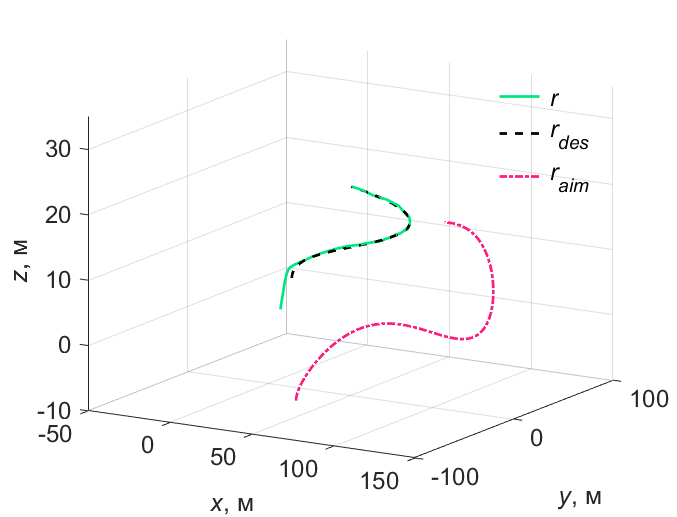
\includegraphics[width=14cm]{traj.png}
	\caption{ -- Траектории: целевая БЛА , пролета БЛА, наблюдаемого объекта}
	\label{fig:mau_traj}
\end{figure}
На рисунке \ref{fig:mau_errors}, слева изображены ошибки ориентации по углам крена, тангажа и рысканья, а справа -- ошибки положения квадрокоптера по осям $X$, $Y$ и $Z$.
Ошибки по каждому из углов ориентации после стабилизации не превышают пяти градусов.
После выхода аппарата на целевую кривую максимальное абсолютное отклонение от траектории составило чуть более полуметра.
\begin{figure}[h!]
	\centering
	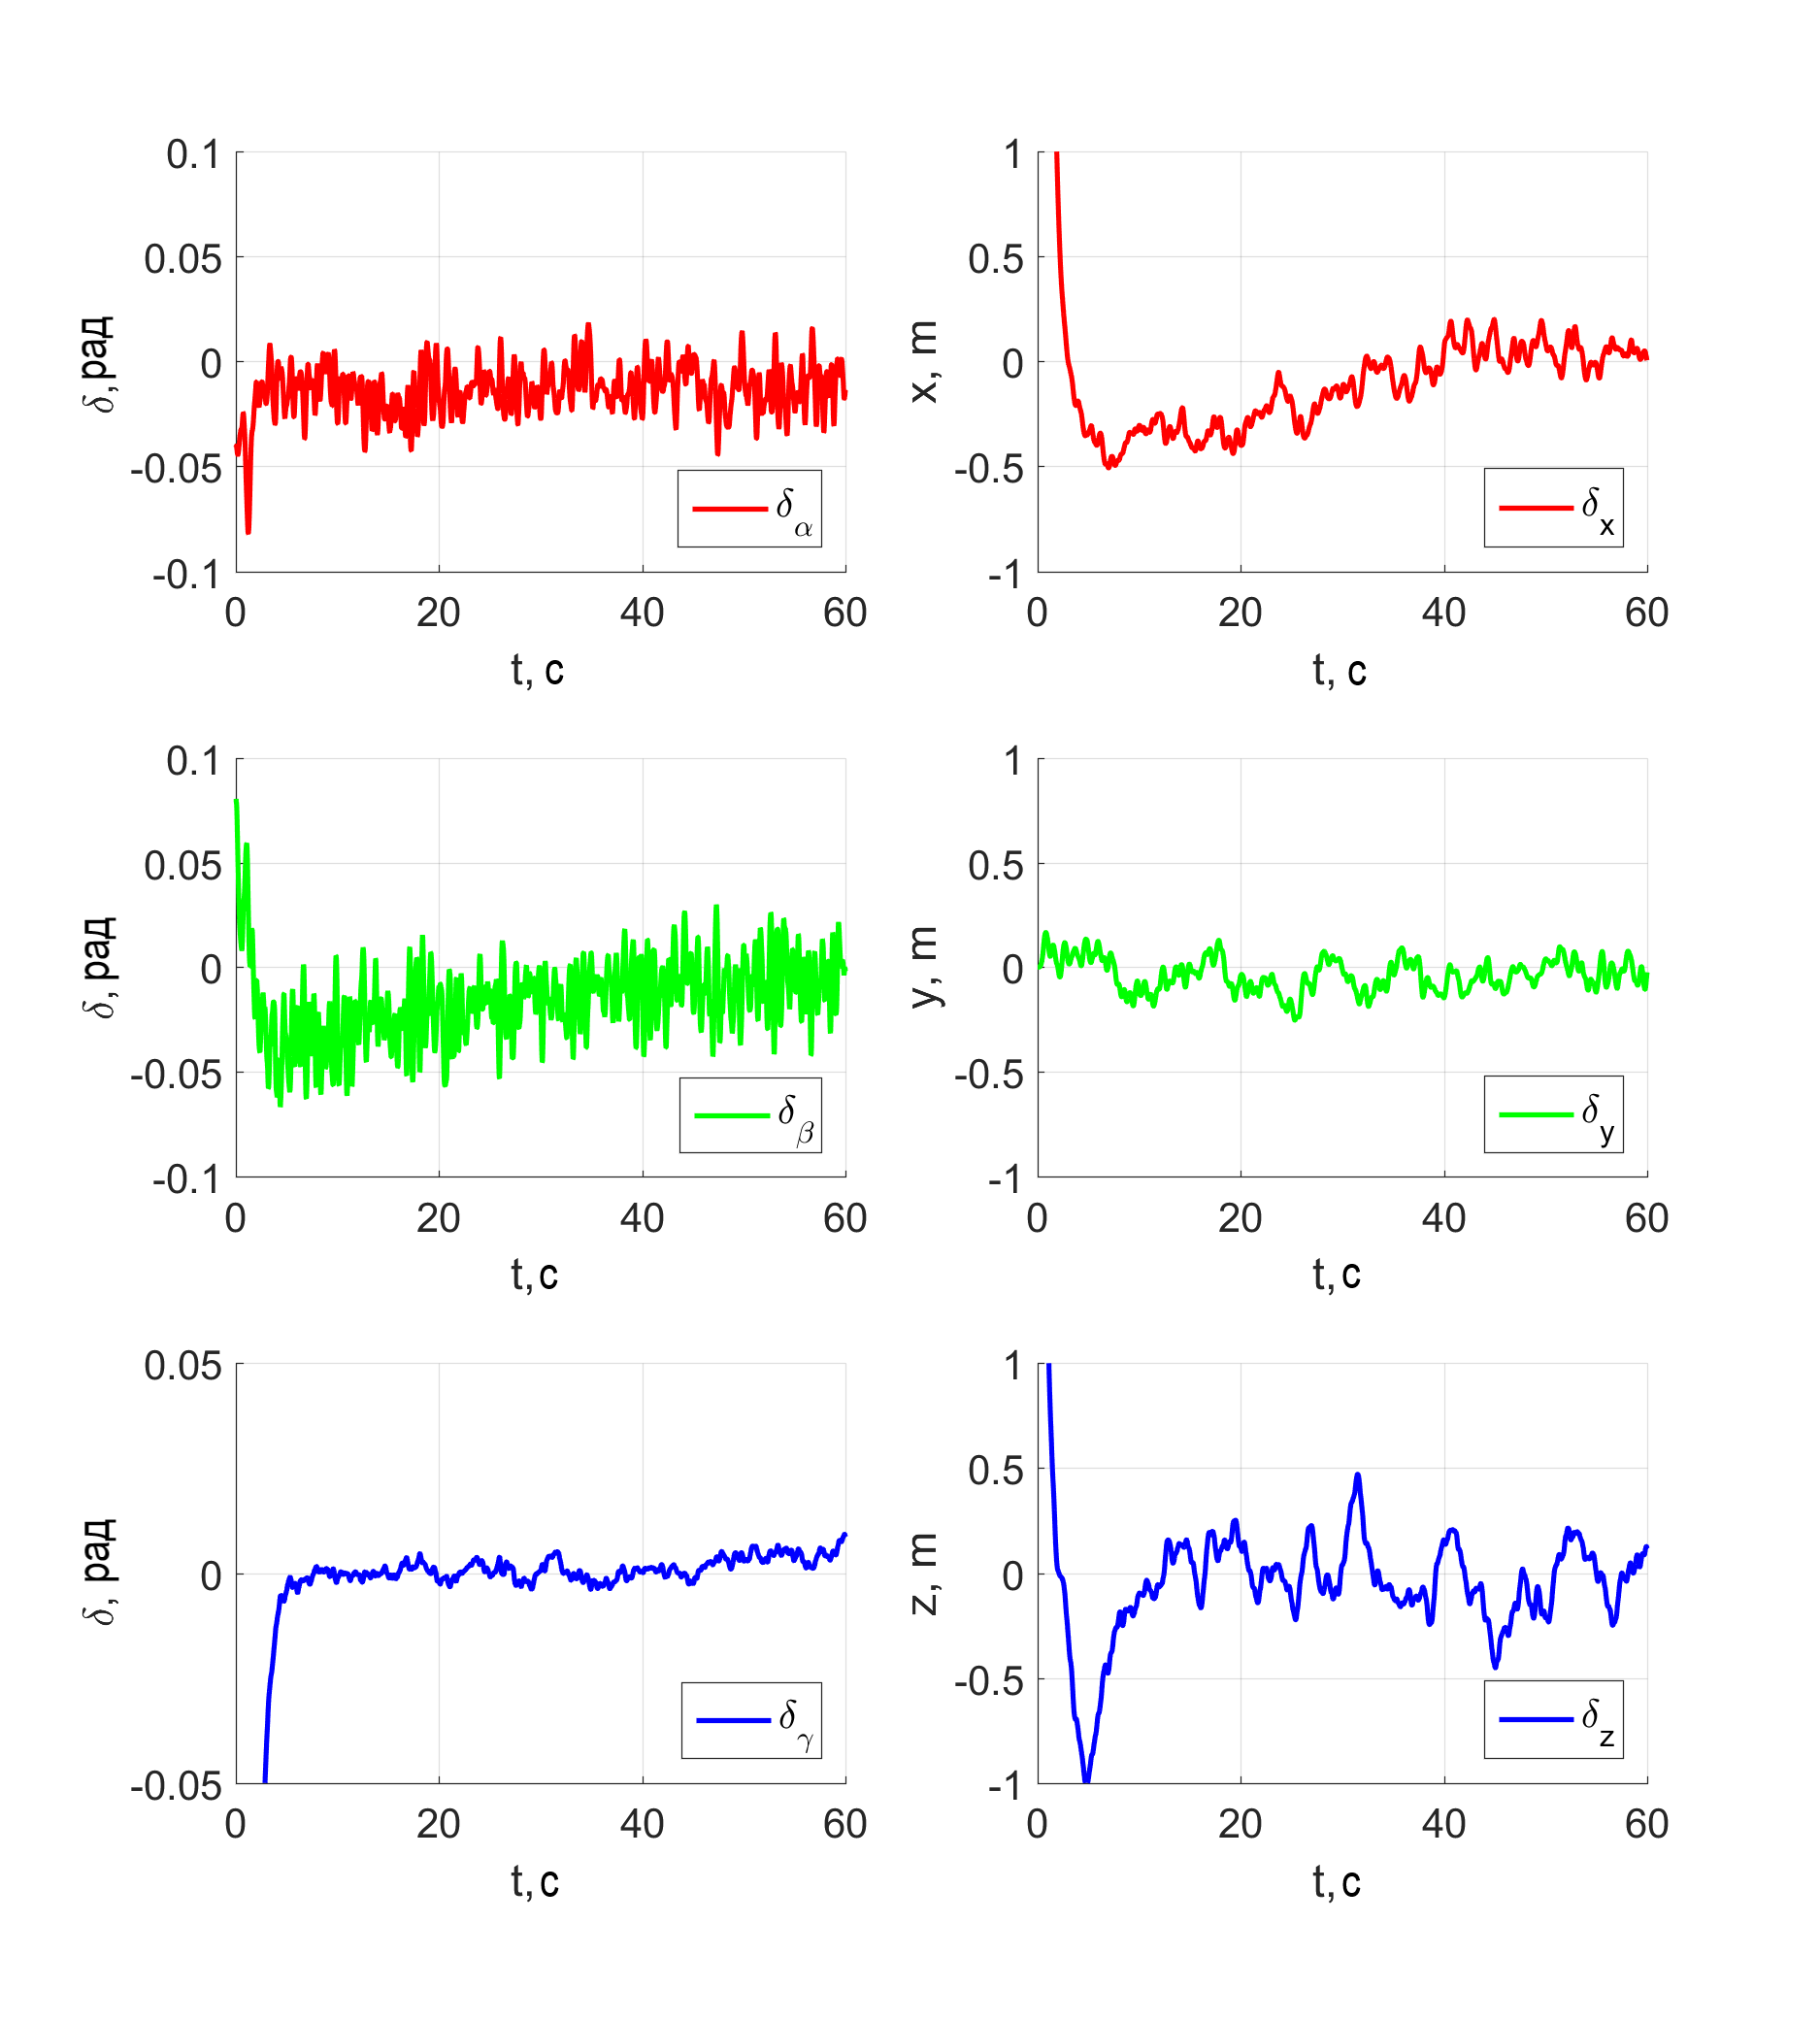
\includegraphics[width=16cm]{errors_rows.png}
	\caption{ -- Ошибка по ориентации и положению}
	\label{fig:mau_errors}
\end{figure}

На рисунке \ref{fig:mau_cam} можно проследить за траекторией наблюдаемого объекта на записи, которою можно сделать с помощью передней камеры.
Видно, что в начальный момент времени объект находится вне зоны видимости, затем перемещается в центр экрана и далее на протяжении всего времени манёвра ось визирования камеры отклоняется от направления на объект не более чем на 4 градуса.
\begin{figure}[h!]
	\centering
	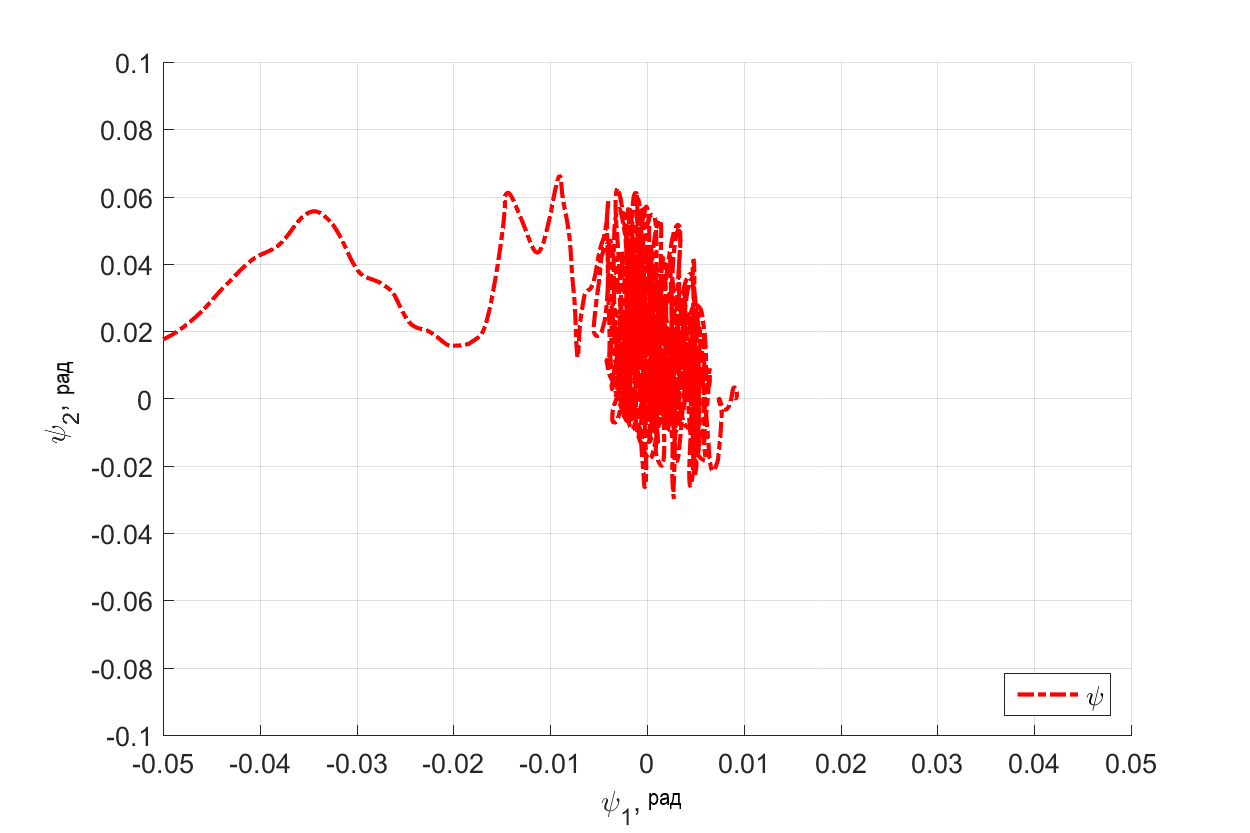
\includegraphics[width=16cm]{camera.png}
	\caption{ -- Траектория объекта на записи}
	\label{fig:mau_cam}
\end{figure}

В результате эксперимента мы оценили способность БЛА с поворотными роторами справляться со сложными маневрами, где необходимо независимо управлять ориентацией и положением аппарата.

\section{Эксперимент: экстренная посадка}

В данном эксперименте рассматривается сценарий отказа двух смежных двигателей. Применяются алгоритмы управления, описанные в разделе \ref{section_em_ctrl}. Как было отмечено, для возможности применения системы экстренного управления необходим значительный запас тяги двигателей и более широкие пределы отклонений сервоприводов. Поэтому в данном эксперименте параметры ограничений БЛА несколько отличаются от тех, что представлены в таблице \ref{tb:params_table}, а именно
\begin{equation}
\begin{aligned}
&\tilde{\omega}_{max} = 1318 \ \text{рад/c},
\\
&\theta_{max} = \pi.
\end{aligned}
\end{equation}

В начальный момент времени аппарат находится на высоте 25 метров недалеко от точки взлета.
При отказе двигателей начинается переход в режим экстренного управления.
За время менее 5 секунд высота БЛА упала более чем на 15 метров, но затем, когда аппарат стабилизировал свою ориентацию около целевых значений, падение прекратилось и аппарат приступил к плавному снижению со скоростью около 0,5 метров в секунду с одновременным движением в сторону места своего запуска.
На рисунке \ref{fig:em_coords} представлены параметры движения мультироторного робота в процессе экстренной посадки. Слева изображены графики компонент векторной части кватерниона ориентации корпуса, справа -- проекции координат центра масс БЛА на оси инерциальной системы отсчета.
\begin{figure}
	\centering
	\subfloat[крен]{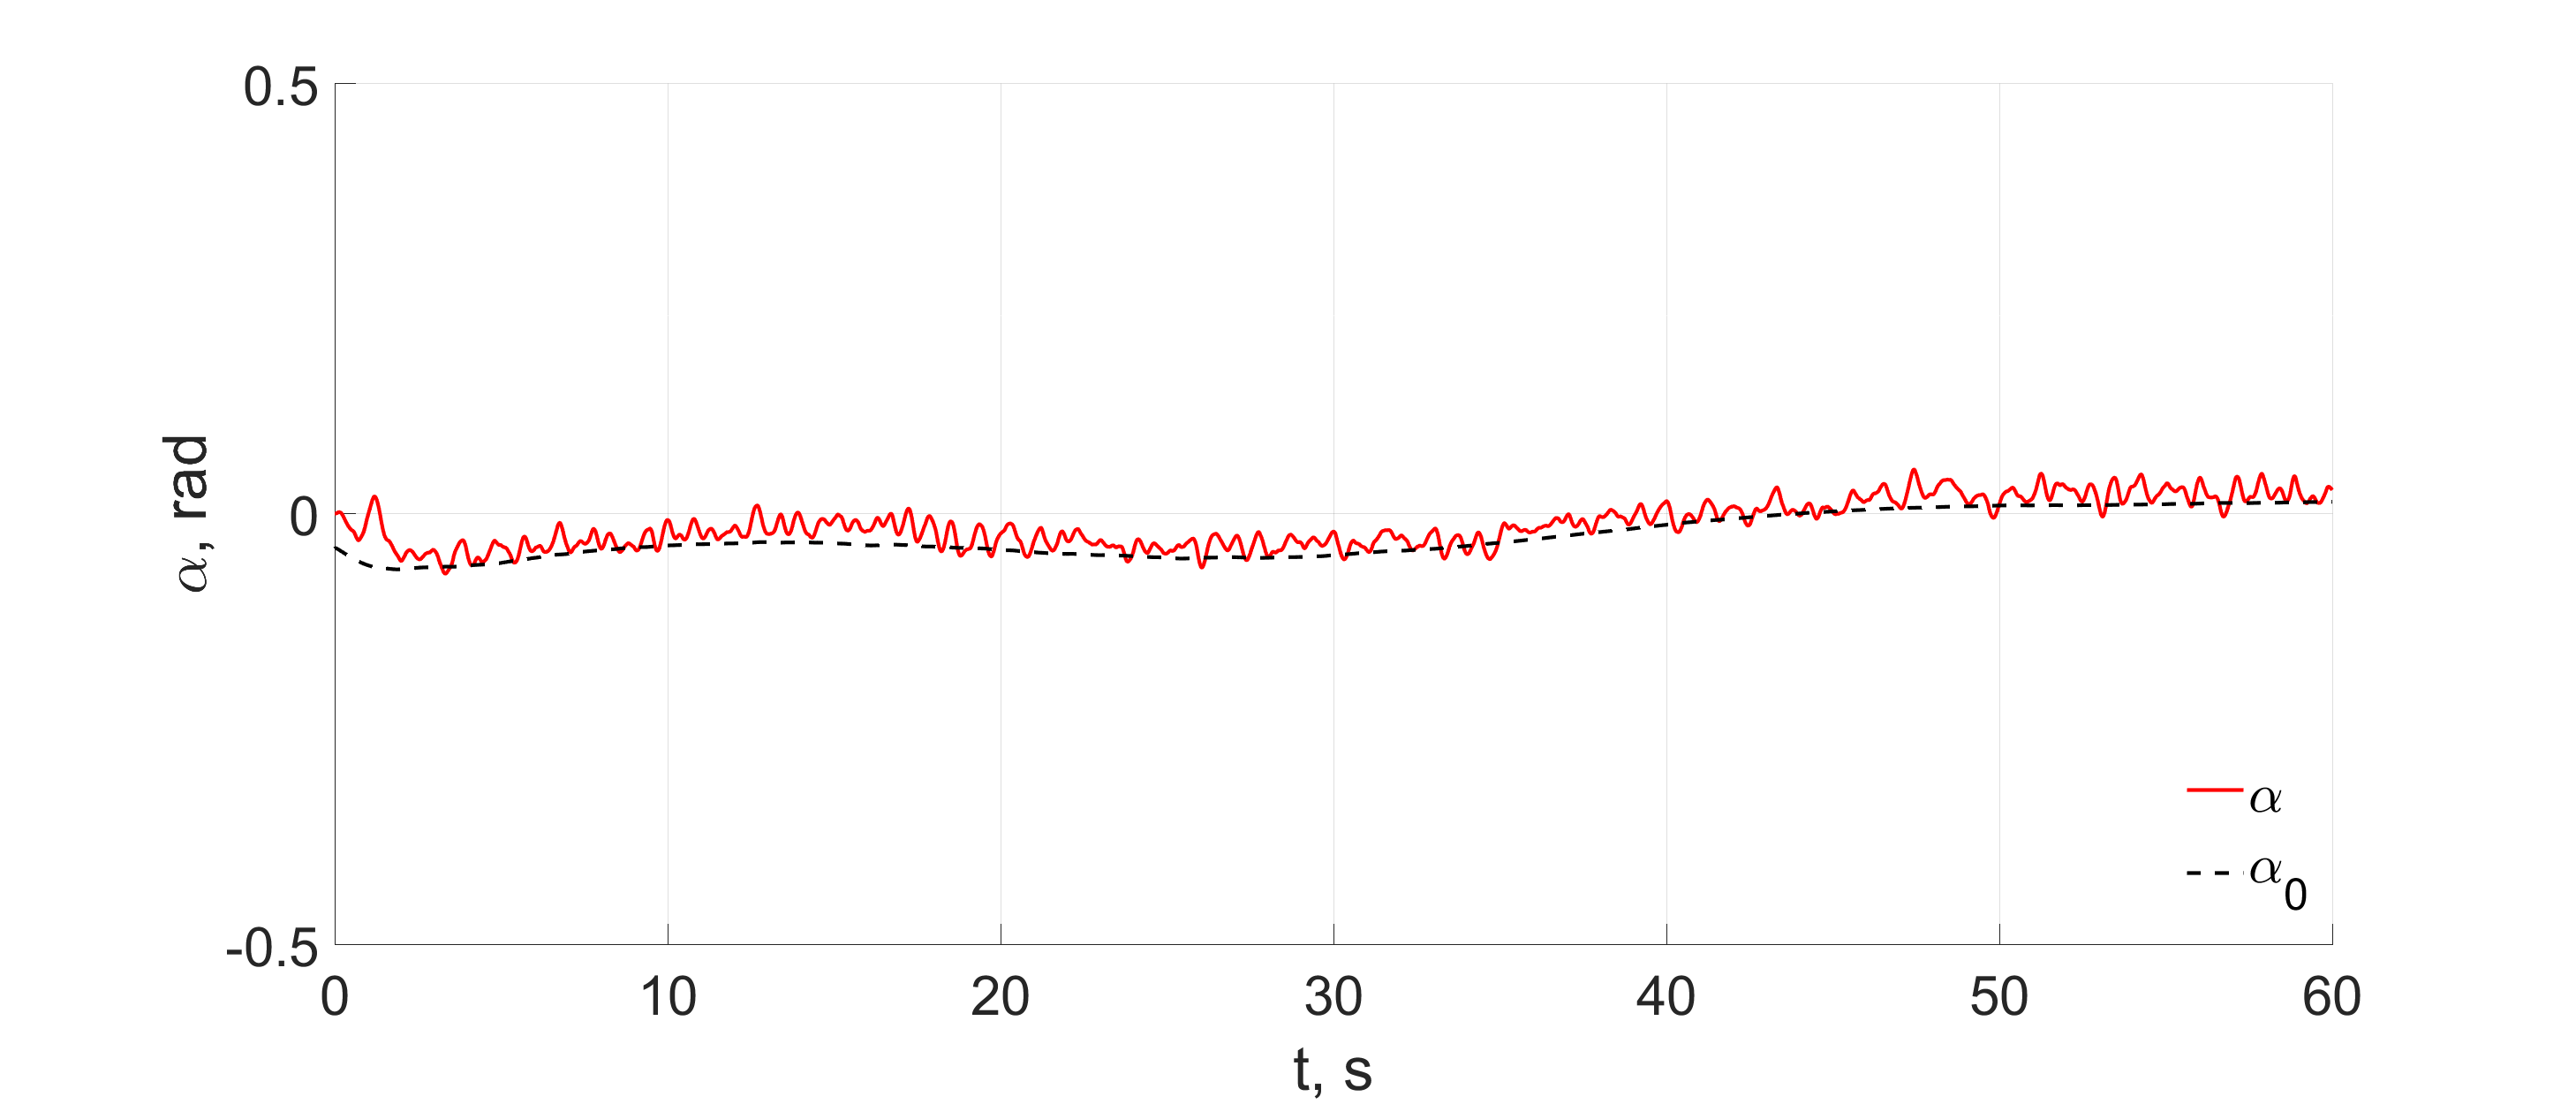
\includegraphics[width=8cm]{em/roll}}\hfil
	\subfloat[координата x]{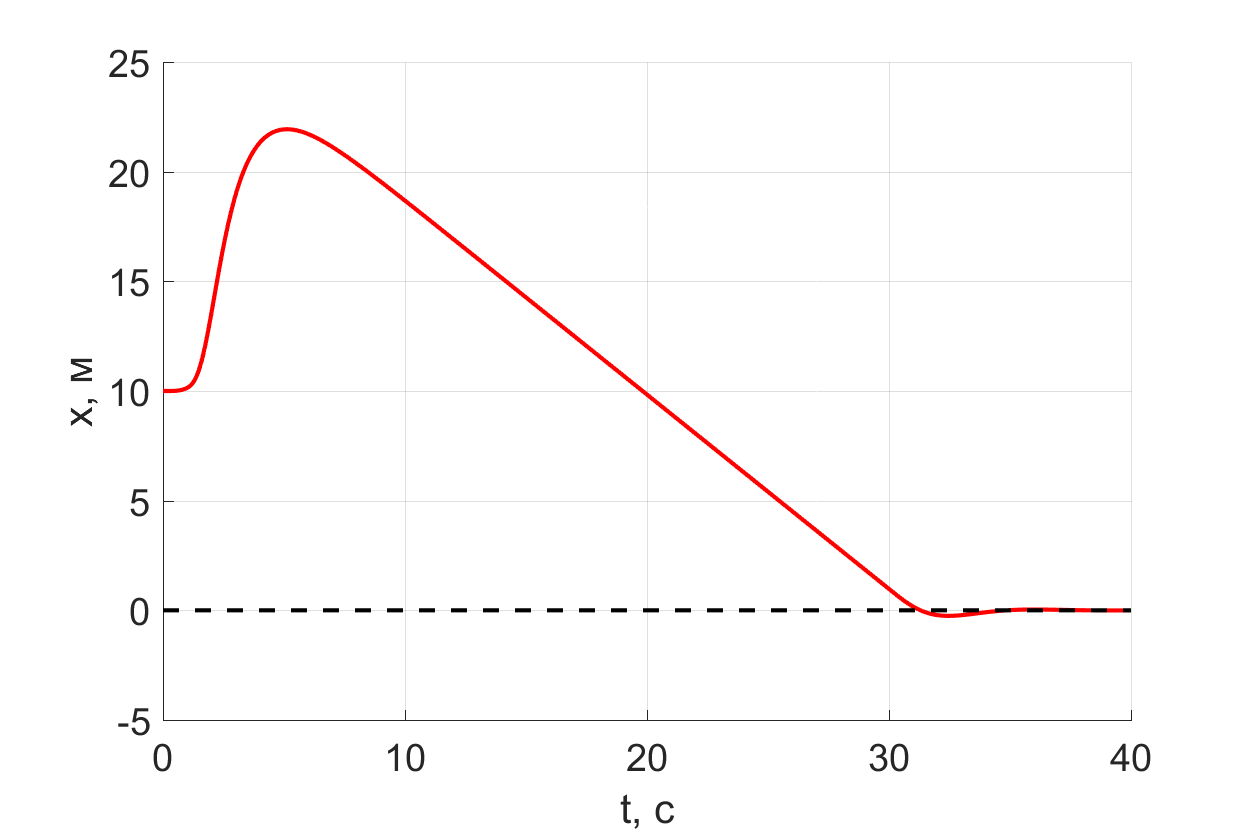
\includegraphics[width=8cm]{em/x}}
	
	\subfloat[тангаж]{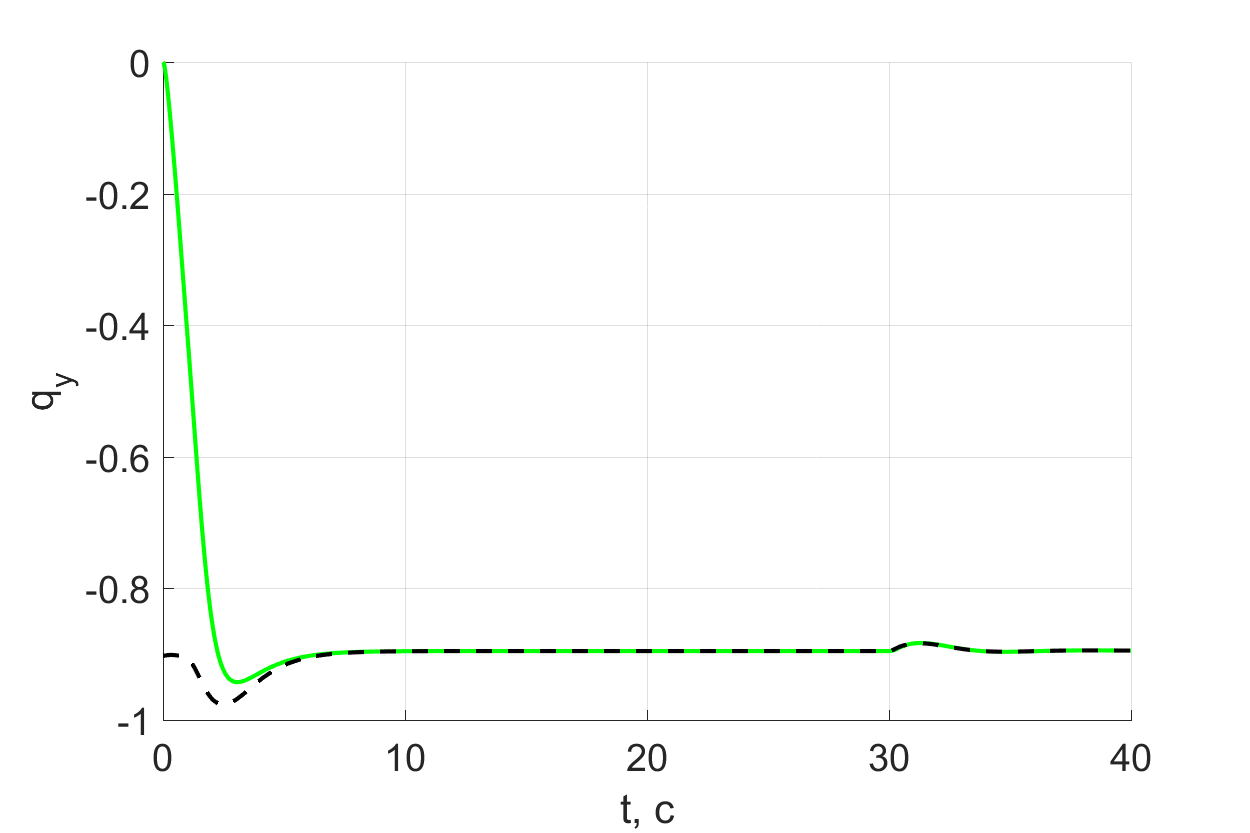
\includegraphics[width=8cm]{em/pitch}} \hfil 
	\subfloat[координата y]{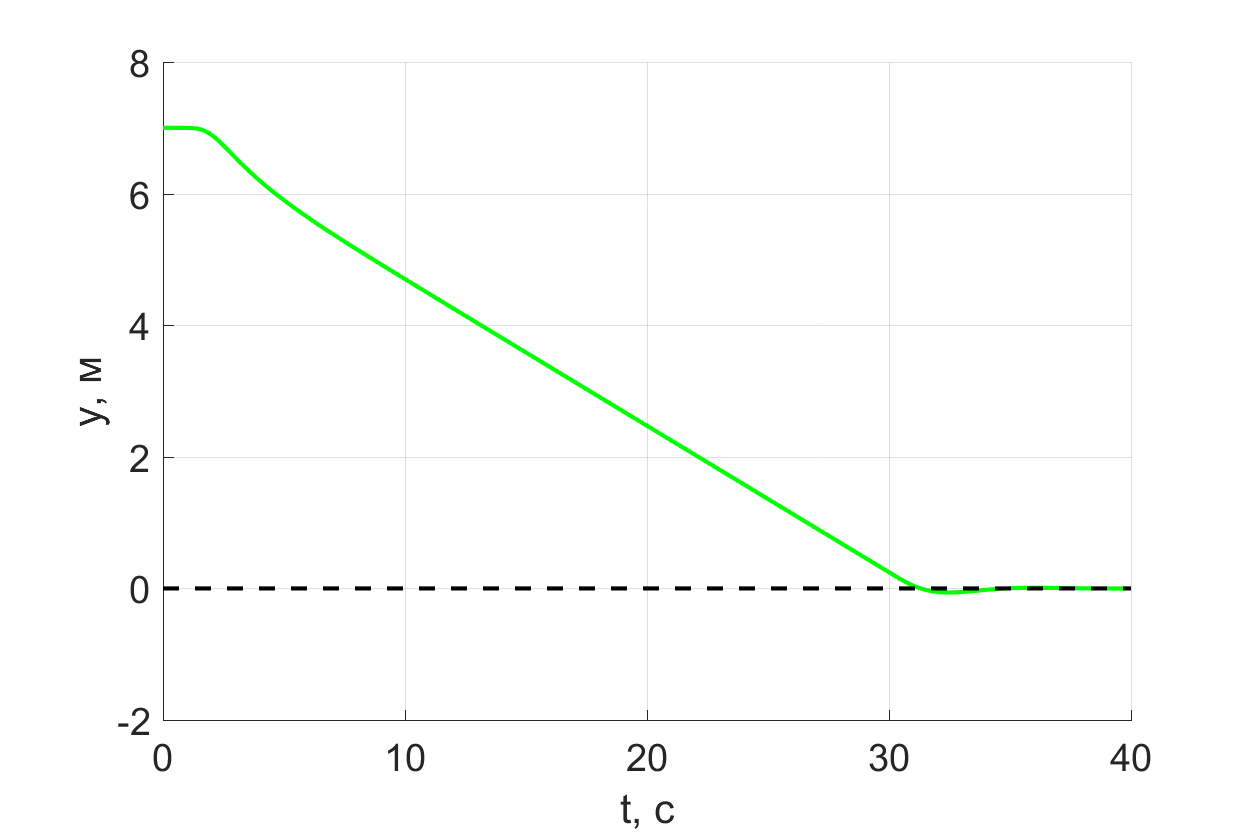
\includegraphics[width=8cm]{em/y}}  
	
	\subfloat[рысканье]{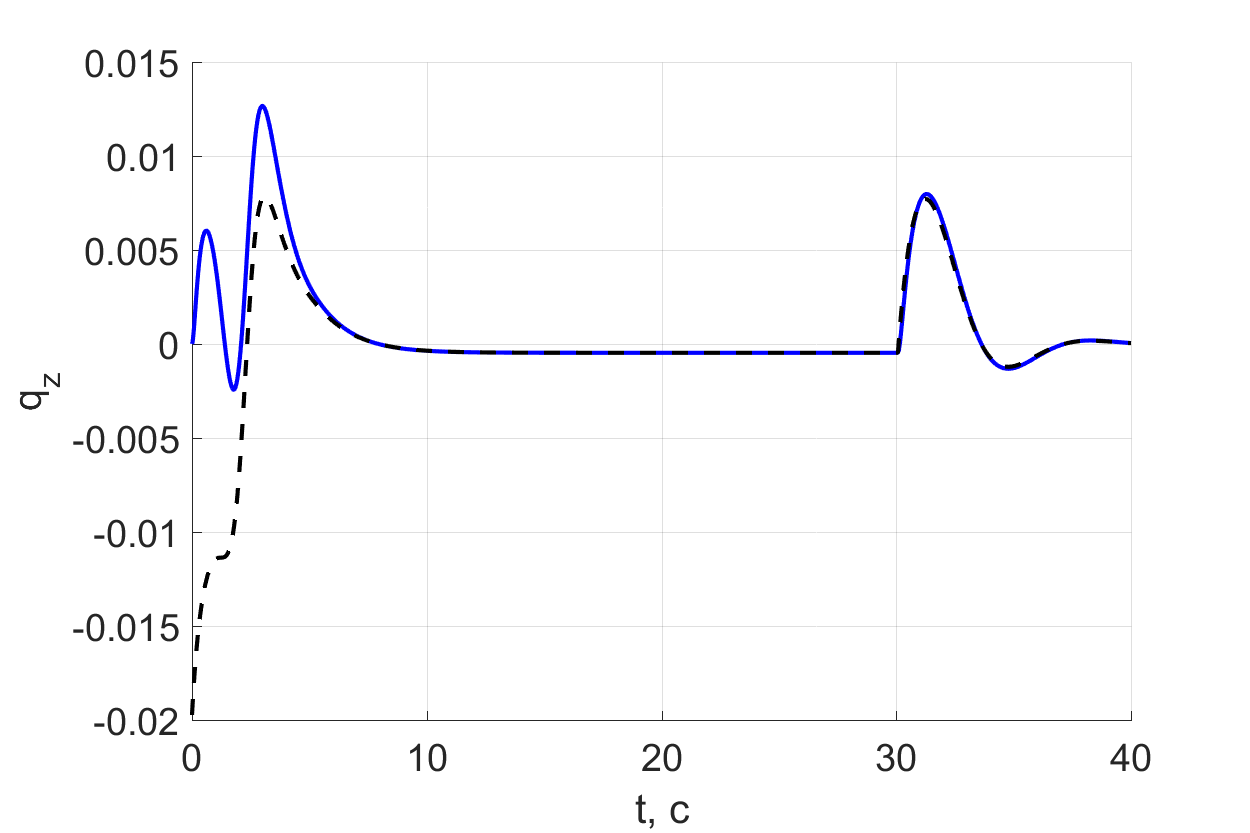
\includegraphics[width=8cm]{em/yaw}}\hfil
	\subfloat[координата z]{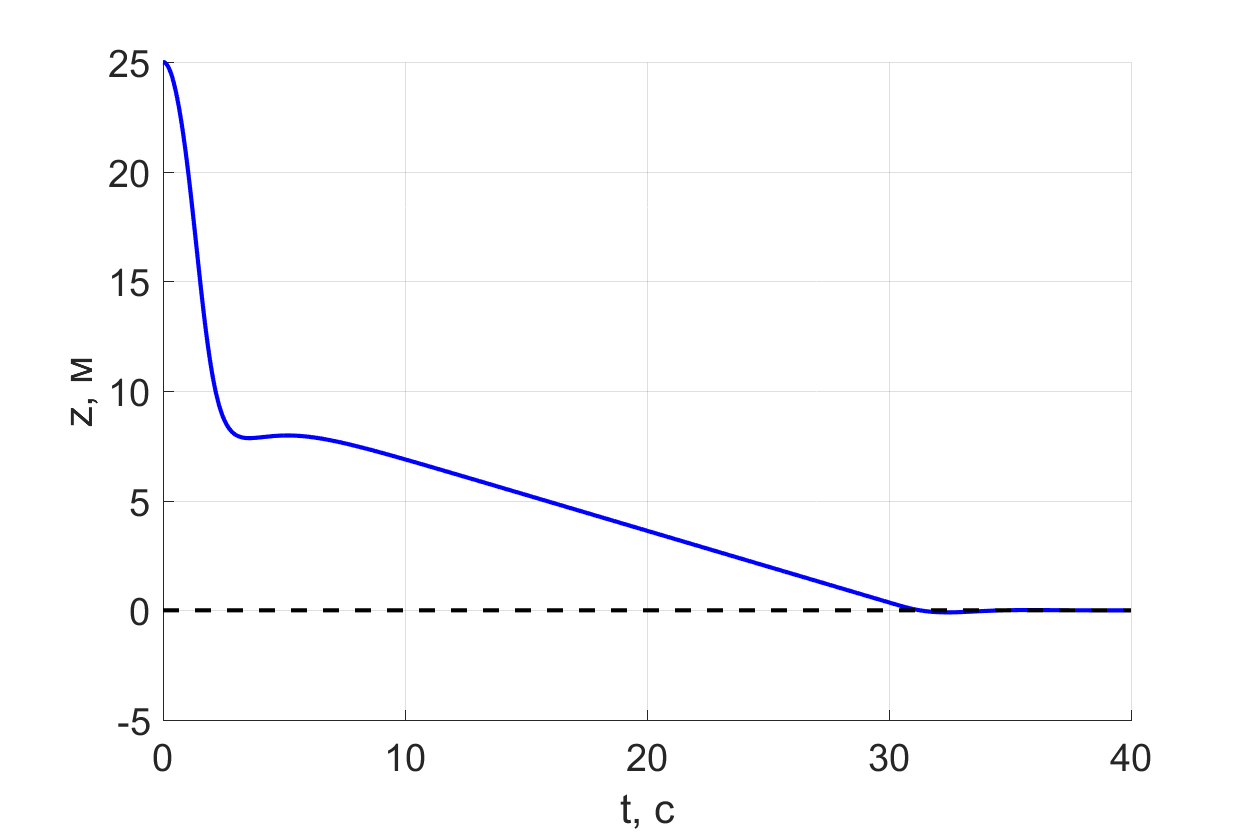
\includegraphics[width=8cm]{em/z}}
	\caption{ -- Параметры движения БЛА при экстренной посадке}
	\label{fig:em_coords}
\end{figure}